\documentclass[tikz, border=4pt]{standalone}
\usepackage{tikz}
\usepackage{karnaugh-map}
\begin{document}
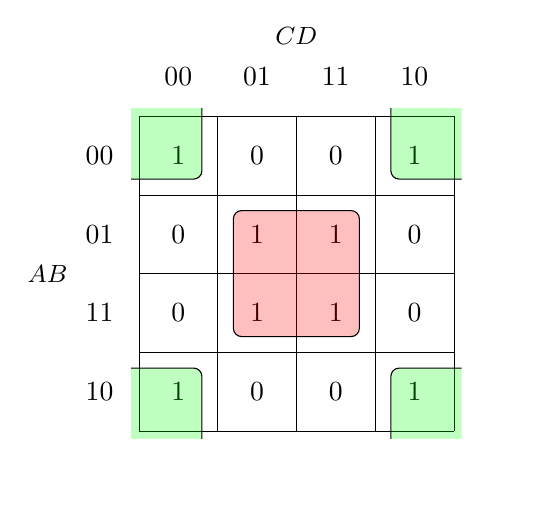
\begin{tikzpicture}[x=1cm, y=1cm]
  \node[inner sep=0pt] at (3.27,-3.11) {\pgfinterruptpicture%
  \begin{karnaugh-map}[4][4][1][$D$][$C$][$B$][$A$]
    \minterms{0,2,5,7,8,10,13,15}
    \autoterms[0]
    \implicant{5}{15}
    \implicantcorner
  \end{karnaugh-map}%
  \endpgfinterruptpicture};
\end{tikzpicture}
\end{document}
